% !TEX program = lualatex
\documentclass[luatexja,ja=standard,a4paper,12pt]{bxjsarticle}

% 数学と図の基本パッケージ
\usepackage{amsmath,amssymb,mathtools,bm}
\usepackage{tikz}
\usetikzlibrary{arrows.meta,calc}
\usepackage{tikz-cd}
\usepackage{enumitem}
\usepackage[unicode]{hyperref}

% 記法
\newcommand{\R}{\mathbb{R}}
\newcommand{\ip}[2]{\left\langle #1,\,#2 \right\rangle}
\newcommand{\vv}[1]{\bm{#1}}

\title{\R$^3$ の順序対構造と内積の基礎\\— Lean 4 形式化と平行四辺形法則 —}
\author{TeX 生成：CODEX (OpenAI)\\Lean 生成：CODEX (OpenAI)}
\date{\today}

\begin{document}
\maketitle

\begin{abstract}
本稿では、ニコラ・ブルバキ『数学原論』の精神に従い、実三次元ベクトル空間
\(\R^3\) を積構造 \(\R \times (\R \times \R)\) として扱い、射影（座標）により
演算を構成する。内積と二乗ノルム、差ベクトル、標準基底の性質を整理し、
平行四辺形法則の証明を座標計算に還元して与える。併せて、Lean 4（mathlib）
による形式化の要点と対応を記す。
\end{abstract}

\section{積と射影による構造}
集合として \(\R^3 \simeq \R \times (\R \times \R)\) と見做し、射影
\(\pi_1,\,\pi_{21},\,\pi_{22}\) を
\[\pi_1(x,(y,z))=x,\qquad \pi_{21}(x,(y,z))=y,\qquad \pi_{22}(x,(y,z))=z\]
と定める。加法、スカラー倍、内積は各成分へ射影して定義される。

\begin{center}
\begin{tikzcd}[row sep=small]
 & \R^3 \simeq \R\times(\R\times\R) \arrow[dl, "\pi_1"'] \arrow[d, "\pi_{21}"] \arrow[dr, "\pi_{22}"] \\
 \R & \R & \R
\end{tikzcd}
\end{center}

\paragraph{演算の定義} ベクトル \(\vv u=(u_1,u_2,u_3)\), \(\vv v=(v_1,v_2,v_3)\) に対し
\begin{align*}
 \vv u+\vv v&:=(u_1+v_1,\,u_2+v_2,\,u_3+v_3),\\
 a\,\vv u&:=(a u_1,\,a u_2,\,a u_3)\quad(a\in\R),\\
 \ip{\vv u}{\vv v}&:=u_1 v_1+u_2 v_2+u_3 v_3,\\
 \mathrm{normSq}(\vv u)&:=\ip{\vv u}{\vv u}=u_1^2+u_2^2+u_3^2,\\
 \mathrm{vec}(\vv A,\vv B)&:=\vv B-\vv A=(B_1-A_1,\,B_2-A_2,\,B_3-A_3).
\end{align*}
標準基底は \(\vv e_1=(1,0,0),\ \vv e_2=(0,1,0),\ \vv e_3=(0,0,1)\) である。

\paragraph{射影と和の可換図式} 各 \(i\in\{1,2,3\}\) について
\begin{center}
\begin{tikzcd}
 \R^3\times\R^3 \arrow[r, "\nabla" ] \arrow[d, "\pi_i\times\pi_i"'] & \R^3 \arrow[d, "\pi_i"] \\
 \R\times\R \arrow[r, "+"'] & \R
\end{tikzcd}
\end{center}
が可換。ここで \(\nabla\) はベクトル和、下段は実数の和である。

\section{基礎問題の計算}
以降、具体ベクトル
\(\,\vv U=(2,-1,0),\ \vv V=(1,3,4),\ \vv A=(1,-2,3),\ \vv B=(4,2,-1)\,\) を用いる。

\begin{enumerate}[label=\textbf{Q\arabic*:},leftmargin=*]
 \item \textbf{差ベクトル} \(\,\mathrm{vec}(\vv A,\vv B)=(3,4,-4)\,\)。\\
 証明：定義展開より \((4-1,\ 2-(-2),\ -1-3)=(3,4,-4)\)。

 \item \textbf{二乗ノルム} \(\,\mathrm{normSq}(\mathrm{vec}(\vv A,\vv B))=3^2+4^2+(-4)^2=41\,\)。

 \item \textbf{線形結合} \(\,2\vv U-3\vv V=(1,-11,-12)\,\)。\\
 成分ごとに \((4-3,\ -2-9,\ 0-12)\) を得る。

 \item \textbf{可換律} 任意の \(\vv u,\vv v\in\R^3\) で \(\vv u+\vv v=\vv v+\vv u\)。

 \item \textbf{基底分解} 任意の \((x,y,z)\in\R^3\) は
 \((x,y,z)=x\,\vv e_1+y\,\vv e_2+z\,\vv e_3\)。

 \item \textbf{基底との内積} \(\ip{(x,y,z)}{\vv e_1}=x\)。\\
 定義より \(x\cdot1+y\cdot0+z\cdot0=x\)。
\end{enumerate}

\section{平行四辺形法則}
任意の \(\vv u,\vv v\in\R^3\) について
\begin{equation}\label{eq:parallelogram}
 \ip{\vv u+\vv v}{\vv u+\vv v}+\ip{\vv u-\vv v}{\vv u-\vv v}
 = 2\,\ip{\vv u}{\vv u}+2\,\ip{\vv v}{\vv v}.
\end{equation}
\paragraph{証明} 成分に分解して一次・二次の項で整理する：
\begin{align*}
 &\ip{\vv u+\vv v}{\vv u+\vv v}+\ip{\vv u-\vv v}{\vv u-\vv v}\\
 &=\sum_{i=1}^3\bigl((u_i+v_i)^2+(u_i-v_i)^2\bigr)
 =\sum_{i=1}^3 2(u_i^2+v_i^2)
 =2\,\ip{\vv u}{\vv u}+2\,\ip{\vv v}{\vv v}.
\end{align*}
各成分で恒等式 \((a+b)^2+(a-b)^2=2(a^2+b^2)\) を用いた。

\begin{center}
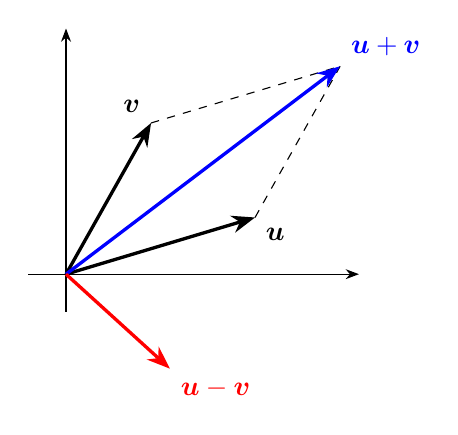
\begin{tikzpicture}[scale=1.2,>=Stealth]
  \coordinate (O) at (0,0);
  \coordinate (U) at (2,0.6);
  \coordinate (V) at (0.9,1.6);
  \coordinate (UPV) at ($(U)+(V)$);
  \coordinate (UminusV) at ($(U)-(V)$);
  % 軸
  \draw[->,thin] (-0.4,0) -- (3.1,0);
  \draw[->,thin] (0,-0.4) -- (0,2.6);
  % ベクトル
  \draw[->,very thick] (O)--(U) node[below right]{$\bm u$};
  \draw[->,very thick] (O)--(V) node[above left]{$\bm v$};
  \draw[dashed] (U)--(UPV) (V)--(UPV);
  \draw[->,very thick,blue] (O)--(UPV) node[above right]{$\bm u+\bm v$};
  \draw[->,very thick,red] (O)--(UminusV) node[below right]{$\bm u-\bm v$};
\end{tikzpicture}
\end{center}

図では平行四辺形の対角線が \(\vv u+\vv v\) と \(\vv u-\vv v\) を与える。

\section{Lean 4 形式化との対応}
本稿の記述は Lean ファイル
\texttt{src/MyProjects/LinearAlgebra/A1/ZenLA1\_Session01.lean} の定理
\texttt{Q1a}〜\texttt{Q5}, \texttt{Challenge} に対応する。証明の要点：
\begin{itemize}
 \item \textbf{座標化（射影）}: `ext` で等式を成分ごとに還元。
 \item \textbf{定義展開}: `simp` で `dot`, `vec`, `e1`〜`e3` を展開。
 \item \textbf{計算整理}: 整数演算は `norm_num`、多項式展開は `ring`/`ring_nf`。
 \item \textbf{Challenge}: `simp [dot, sub_eq_add_neg, ...]` の後に `ring`。
\end{itemize}

\paragraph{再現手順} \texttt{lake build} でビルドし、VS Code なら Lean サーバ上で
各定理のゴールビューを確認できる。内積記法を係数の右因子に置くときは
括弧で明示（例：\( (2:\R)\cdot(\ip{\vv u}{\vv u}) \)）。

\section*{謝辞と生成に関する明示}
この TeX 文書および対応する Lean ファイルは、CODEX (OpenAI) により生成されました。
著者表記として「TeX 生成：CODEX (OpenAI)、Lean 生成：CODEX (OpenAI)」と明示します。

\end{document}

